\documentclass[aspectratio=169,14pt]{beamer}
\usetheme{default}
\usepackage{fontspec}
\setmainfont{texgyrepagella-regular.otf}[BoldFont=texgyrepagella-bold.otf,ItalicFont=texgyrepagella-italic.otf,BoldItalicFont=texgyrepagella-bolditalic.otf]
\setsansfont{texgyreheros-regular.otf}[BoldFont=texgyreheros-bold.otf,ItalicFont=texgyreheros-italic.otf,BoldItalicFont=texgyreheros-bold.otf,BoldItalicFeatures={FakeSlant=0.2}]
\setmonofont{lmmono10-regular.otf}[Scale=0.85]
\setbeamertemplate{navigation symbols}{}
\usepackage{pgfpages}
\newif\ifpresenter
\ifdefined\PresenterVersion\presentertrue\else\presenterfalse\fi
\ifpresenter
  \setbeameroption{show notes on second screen=right}
  \setbeamertemplate{note page}[plain]
\fi
\usepackage{amsmath,amssymb,bm,booktabs,array,graphicx,xcolor}
\usepackage{tikz,pgfplots,adjustbox,listings,xurl}
\pgfplotsset{compat=1.18}
\usetikzlibrary{arrows.meta,positioning,calc,fit,shapes.geometric,decorations.pathreplacing,patterns}
% UIUC official brand colors, verified 2026-10-23.
% https://brand.illinois.edu/visual-identity/color
\definecolor{IlliniOrange}{HTML}{FF5F05}
\definecolor{IlliniBlue}{HTML}{13294B}
\definecolor{Storm}{HTML}{707372}
\definecolor{LightStorm}{HTML}{C6C7C6}
\definecolor{Industrial}{HTML}{1D58A7}
\definecolor{Patina}{HTML}{007E8E}
\tikzset{>=Stealth, every node/.style={font=\small,text=IlliniBlue}, box/.style={draw=IlliniBlue,rounded corners=2pt,align=center,inner sep=6pt,execute at begin node=\hyphenpenalty10000\relax}, orangebox/.style={box,draw=IlliniOrange,very thick}, edge/.style={->,thick,IlliniBlue}, accent/.style={->,very thick,IlliniOrange}}
\pgfplotsset{every axis/.append style={width=13.5cm,height=6.5cm,axis line style={IlliniBlue},tick label style={font=\small,text=IlliniBlue},label style={font=\small,text=IlliniBlue},legend style={font=\small,draw=none,fill=white},grid style={LightStorm},major grid style={LightStorm},axis lines=left,clip=false}, every axis plot/.append style={thick}}

\definecolor{slidepaper}{RGB}{234,220,201}
\setbeamercolor{background canvas}{bg=slidepaper}
\setbeamercolor{normal text}{fg=IlliniBlue}
\setbeamercolor{frametitle}{fg=IlliniBlue}
\setbeamercolor{title}{fg=IlliniBlue}
\setbeamercolor{item}{fg=IlliniOrange}
\setbeamerfont{frametitle}{size=\large,series=\bfseries}
\setbeamerfont{title}{size=\Large,series=\bfseries}
\setbeamertemplate{itemize item}{\color{IlliniOrange}$\bullet$}
\setbeamertemplate{itemize subitem}{\color{IlliniOrange}\footnotesize$\circ$}
\setbeamercolor{orangerule}{bg=IlliniOrange}
\setbeamertemplate{headline}{\begin{beamercolorbox}[wd=\paperwidth,ht=0.1cm,dp=0.1cm]{orangerule}\end{beamercolorbox}}
\setbeamertemplate{footline}{\begin{beamercolorbox}[wd=\paperwidth,ht=0.1cm,dp=0.1cm]{orangerule}\end{beamercolorbox}}
\setbeamersize{text margin left=0.65cm,text margin right=0.65cm}
\setlength{\leftmargini}{1.1em}
\newenvironment{slidebullets}{\begin{itemize}\setlength\itemsep{0.8em}}{\end{itemize}}
\pgfplotsset{every axis/.append style={legend style={fill=slidepaper}}}
\lstdefinelanguage{CoursePython}{keywords={from,import,for,in,if,else,def,return,assert,True,False,None},sensitive=true,morecomment=[l]{\#},morestring=[b]',morestring=[b]"}
\lstset{language=CoursePython,basicstyle=\ttfamily\small,keywordstyle=\color{IlliniBlue}\bfseries,commentstyle=\color{Storm},stringstyle=\color{IlliniBlue},showstringspaces=false,breaklines=true,columns=fullflexible,keepspaces=true,frame=none,aboveskip=0.7em,belowskip=0.7em}
\newcommand{\E}{\mathbb E}
\newcommand{\Var}{\operatorname{Var}}
\newcommand{\Cov}{\operatorname{Cov}}
\hypersetup{colorlinks=true,urlcolor=IlliniBlue,linkcolor=IlliniBlue}

\title{Marketing Analytics}
\subtitle{Recommendation Systems and Customer Goals}
\author{By Nathan Yang}
\date{Session 12}
\begin{document}
\begin{frame}
\titlepage
\end{frame}
\begin{frame}{A Returning-Customer Decision}
\usebeamercolor[fg]{normal text}
\vfill
\begin{slidebullets}
\item An mHealth user returns to log a meal.
\item The system chooses among eligible categories using earlier histories.
\item The objective may include familiar relevance and a stated variety goal.
\end{slidebullets}
\vfill
\note{The next logged basket differs from the next item row. A basket can contain several relevant categories. Availability and the customer's goal constrain which recommendations are useful.

M7, Section 7.15, Marketing Analytics Lecture Notes. \url{../06_Lecture_Notes/modules/M07_Prediction_and_Machine_Learning.md}}
\end{frame}
\begin{frame}{The Candidate Set}
\usebeamercolor[fg]{normal text}
\vfill
\begin{slidebullets}
\item Candidate generation determines what can be recommended.
\item Scoring compares eligible items using current information.
\item Ranking chooses order and applies list constraints.
\end{slidebullets}
\vfill
\note{A strong ranking model cannot recover an item excluded during candidate generation. Evaluation must retain the candidate-set definition as well as the ranked output.

M7, Section 7.10, Marketing Analytics Lecture Notes. \url{../06_Lecture_Notes/modules/M07_Prediction_and_Machine_Learning.md}}
\end{frame}
\begin{frame}{Recommendation Models}
\usebeamercolor[fg]{normal text}
\vfill
\begin{slidebullets}
\item Content models compare item attributes and customer histories.
\item Collaborative models learn patterns across customers and items.
\item Popularity and personal-frequency rules provide useful baselines.
\end{slidebullets}
\vfill
\note{A content model can help with new items that lack interactions. A collaborative model benefits from shared behavior but faces cold-start and selected-exposure problems.

M7, Section 7.10, Marketing Analytics Lecture Notes. \url{../06_Lecture_Notes/modules/M07_Prediction_and_Machine_Learning.md}}
\end{frame}
\begin{frame}{Histories Must Precede the Basket}
\usebeamercolor[fg]{normal text}
\centering
\begingroup
\fontsize{11}{13.2}\selectfont
\def\small{\fontsize{10}{12}\selectfont}
\def\footnotesize{\fontsize{9}{11}\selectfont}
\def\scriptsize{\fontsize{8}{9.5}\selectfont}
\hyphenpenalty=10000
\begin{adjustbox}{max width=0.98\textwidth,max totalheight=0.65\textheight}
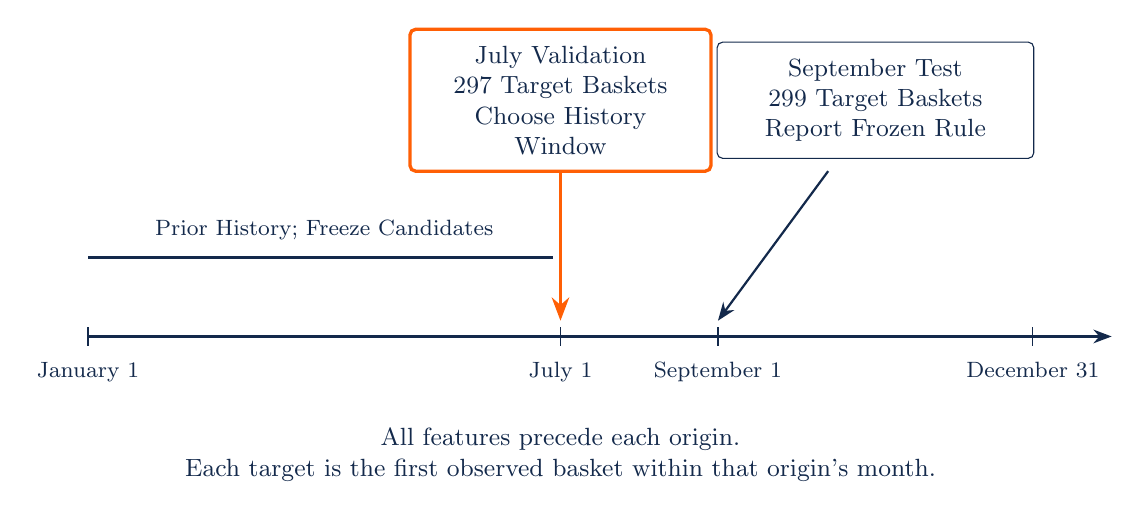
\begin{tikzpicture}[x=1cm,y=1cm]
\draw[edge] (0,0)--(13,0);
\foreach \x/\label in {0/January 1,6/July 1,8/September 1,12/December 31}{\draw[IlliniBlue] (\x,.12)--(\x,-.12);\node[anchor=north,font=\footnotesize] at (\x,-.2) {\label};}
\draw[IlliniBlue,very thick] (0,1)--(5.9,1);
\node[anchor=south,font=\footnotesize] at (3,1.1) {Prior History; Freeze Candidates};
\node[orangebox,text width=3.4cm] at (6,3.0) {July Validation\\297 Target Baskets\\Choose History Window};
\draw[accent] (6,2.1)--(6,.2);
\node[box,text width=3.6cm] at (10,3.0) {September Test\\299 Target Baskets\\Report Frozen Rule};
\draw[edge] (9.4,2.1)--(8,.2);
\node[align=center,text width=12cm] at (6,-1.5) {All features precede each origin.\\Each target is the first observed basket within that origin's month.};
\end{tikzpicture}

\end{adjustbox}
\endgroup
\par\medskip
{\small mHealth evaluation freezes histories and candidate sets at the forecast origin.\par}
\note{Returning-user prediction can use the user's earlier history while holding out later baskets. The distinction is temporal rather than necessarily a complete user holdout.

M7, Section 7.15.1, Marketing Analytics Lecture Notes. \url{../06_Lecture_Notes/modules/M07_Prediction_and_Machine_Learning.md}}
\end{frame}
\begin{frame}{Recall Among Relevant Categories}
\usebeamercolor[fg]{normal text}
\noindent Let $L_i$ be the top-k list and $B_i$ the categories in the next observed basket.
\medskip
\[
\operatorname{Recall@k}_i=\frac{|L_i\cap B_i|}{|B_i|}
\]
\medskip
\noindent The denominator is the number of relevant basket categories for that user-event.
\note{Report how empty baskets and unavailable categories are handled. Average per event or per user according to the target population, and retain the chosen weighting rule.

M7, Section 7.11, Marketing Analytics Lecture Notes. \url{../06_Lecture_Notes/modules/M07_Prediction_and_Machine_Learning.md}}
\end{frame}
\begin{frame}{Position Matters}
\usebeamercolor[fg]{normal text}
\noindent Discount lower-ranked relevant items when their positions affect exposure.
\medskip
\[
\operatorname{DCG@k}=\sum_{r=1}^{k}\frac{2^{\mathrm{rel}_r}-1}{\log_2(r+1)}
\]
\medskip
\noindent NDCG divides by the best attainable DCG for the same relevance labels.
\note{NDCG depends on the candidate set and relevance definition. Unobserved engagement is not necessarily a negative preference label because exposure is selective.

M7, Section 7.11, Marketing Analytics Lecture Notes. \url{../06_Lecture_Notes/modules/M07_Prediction_and_Machine_Learning.md}}
\end{frame}
\begin{frame}{Basket Associations}
\usebeamercolor[fg]{normal text}
\vfill
\begin{slidebullets}
\item Support counts how often items occur together.
\item Confidence conditions on the antecedent item.
\item Lift compares confidence with the consequent's marginal prevalence.
\end{slidebullets}
\vfill
\note{Association rules are descriptive. A positive lift can reflect common meal occasions or other causes rather than a response to recommendation. Evaluate rules on later baskets.

M7, Section 7.17, Marketing Analytics Lecture Notes. \url{../06_Lecture_Notes/modules/M07_Prediction_and_Machine_Learning.md}}
\end{frame}
\begin{frame}{Lift Changes the Baseline Comparison}
\usebeamercolor[fg]{normal text}
\centering
\begingroup
\begin{adjustbox}{max width=0.98\textwidth,max totalheight=0.65\textheight}
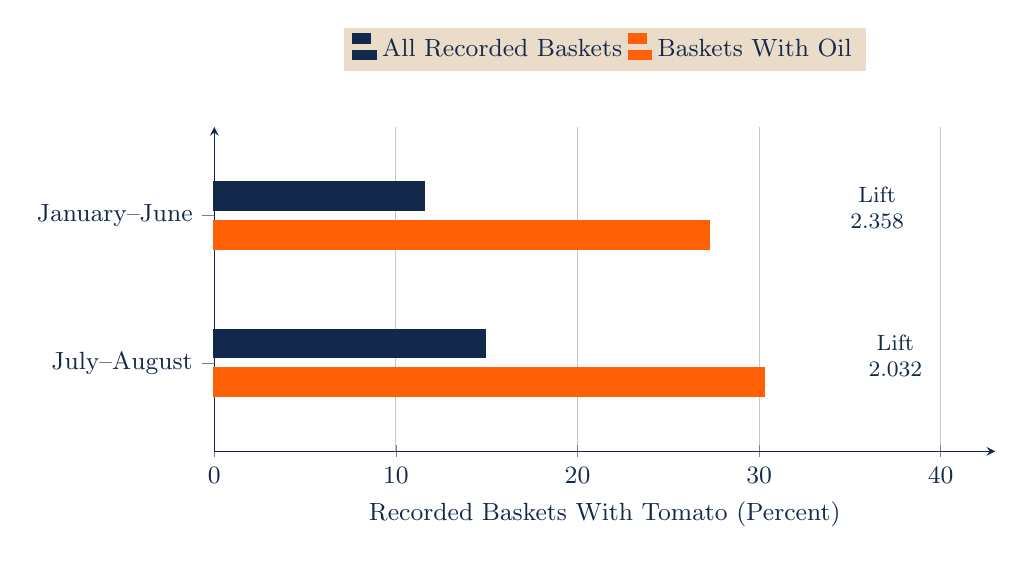
\begin{tikzpicture}
\begin{axis}[xbar,bar width=10pt,width=11.5cm,height=5.7cm,xlabel={Recorded Baskets With Tomato (Percent)},xmin=0,xmax=43,ymin=.4,ymax=2.6,ytick={1,2},yticklabels={July--August,January--June},xtick={0,10,20,30,40},xmajorgrids=true,legend style={at={(.5,1.17)},anchor=south,legend columns=2}]
\addplot[IlliniBlue,fill=IlliniBlue,bar shift=7pt] coordinates {(11.559899,2)(14.896573,1)};
\addlegendentry{All Recorded Baskets}
\addplot[IlliniOrange,fill=IlliniOrange,bar shift=-7pt] coordinates {(27.255252,2)(30.266789,1)};
\addlegendentry{Baskets With Oil}
\node[align=center,font=\footnotesize] at (axis cs:36.5,2.05) {Lift\\2.358};
\node[align=center,font=\footnotesize] at (axis cs:37.5,1.05) {Lift\\2.032};
\end{axis}\end{tikzpicture}

\end{adjustbox}
\endgroup
\par\medskip
{\small mHealth basket rules use distinct baskets and future validation.\par}
\note{Counting item rows instead of distinct baskets changes the denominator and can inflate associations through repeated entries.

M7, Section 7.17, Marketing Analytics Lecture Notes. \url{../06_Lecture_Notes/modules/M07_Prediction_and_Machine_Learning.md}}
\end{frame}
\begin{frame}{Relevance and a Customer Goal}
\usebeamercolor[fg]{normal text}
\noindent Combine relevance $s_j$ with a goal score $g_j$ using an explicit weight.
\medskip
\[
v_j(\alpha)=(1-\alpha)s_j+\alpha g_j
\]
\medskip
\noindent The scores need a comparable scale before the weight has a clear interpretation.
\note{A goal score should reflect a defined customer objective and validated measurement. The weight does not become a preference estimate merely because a programmer sets it.

M7, Section 7.12.1, Marketing Analytics Lecture Notes. \url{../06_Lecture_Notes/modules/M07_Prediction_and_Machine_Learning.md}}
\end{frame}
\begin{frame}{Small Weight Changes Can Change the First Item}
\usebeamercolor[fg]{normal text}
\centering
\begingroup
\begin{adjustbox}{max width=0.98\textwidth,max totalheight=0.65\textheight}
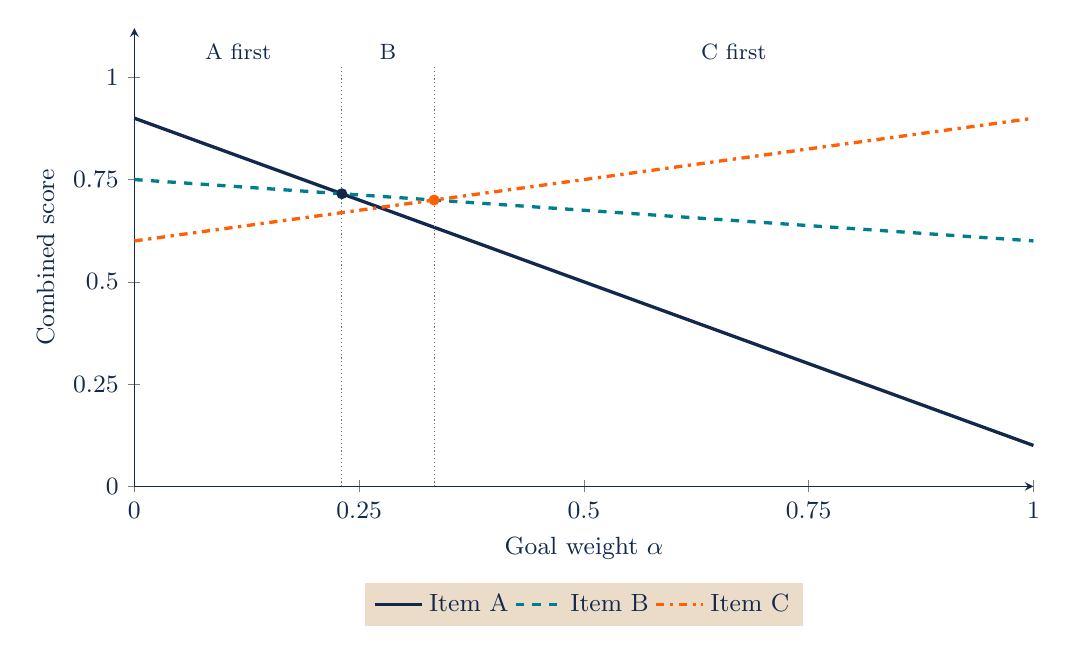
\begin{tikzpicture}
\begin{axis}[width=13cm,height=7.4cm,xmin=0,xmax=1,ymin=0,ymax=1.12,
  xtick={0,.25,.5,.75,1},ytick={0,.25,.5,.75,1},
  xlabel={Goal weight $\alpha$},ylabel={Combined score},
  legend style={at={(.5,-.21)},anchor=north,legend columns=3}]
\addplot[IlliniBlue,very thick,domain=0:1,samples=2]{.9-.8*x};
\addplot[Patina,very thick,dashed,domain=0:1,samples=2]{.75-.15*x};
\addplot[IlliniOrange,very thick,dashdotted,domain=0:1,samples=2]{.6+.3*x};
\legend{Item A,Item B,Item C}
\draw[Storm,densely dotted] (axis cs:.230769,0)--(axis cs:.230769,1.03);
\draw[Storm,densely dotted] (axis cs:.333333,0)--(axis cs:.333333,1.03);
\node[font=\footnotesize,anchor=south] at (axis cs:.1154,1.02) {A first};
\node[font=\footnotesize,anchor=south] at (axis cs:.2821,1.02) {B};
\node[font=\footnotesize,anchor=south] at (axis cs:.6667,1.02) {C first};
\fill[IlliniBlue] (axis cs:.230769,.715385) circle (2pt);
\fill[IlliniOrange] (axis cs:.333333,.7) circle (2pt);
\end{axis}
\end{tikzpicture}

\end{adjustbox}
\endgroup
\par\medskip
{\small Synthetic item scores. Relevance and goal scores stay fixed.\par}
\note{A recommendation can be discontinuous in a tuning weight. Sensitivity analysis should report the ranking itself, not only smooth average scores.

M7, Section 7.12.1, Marketing Analytics Lecture Notes. \url{../06_Lecture_Notes/modules/M07_Prediction_and_Machine_Learning.md}}
\end{frame}
\begin{frame}[fragile]{A Three-Item Basket Check}
\usebeamercolor[fg]{normal text}
\noindent The list contains A, B, and C. The basket contains A and C.
\begin{lstlisting}
from math import log2
ranked = ['A', 'B', 'C']
relevant = {'A', 'C'}
recall = len(set(ranked) & relevant) / len(relevant)
dcg = sum((x in relevant) / log2(r+2)
          for r,x in enumerate(ranked))
ideal = 1 + 1/log2(3)
assert recall == 1.0
\end{lstlisting}
{\small Recall is 1.0, while NDCG is about 0.920 because B occupies the second position.\par}
\note{The calculation uses binary relevance. It assumes all relevant items are eligible and that the observation window defines a valid basket.

M7, Section 7.11, Marketing Analytics Lecture Notes. \url{../06_Lecture_Notes/modules/M07_Prediction_and_Machine_Learning.md}}
\end{frame}
\begin{frame}{LLM Explanations}
\usebeamercolor[fg]{normal text}
\vfill
\begin{slidebullets}
\item Explain a recommendation using verified item attributes.
\item Check whether stated reasons are factually supported.
\item Evaluate explanation effects separately from ranking quality.
\end{slidebullets}
\vfill
\note{An explanation can sound plausible while inventing a nutritional property or claiming a nonexistent personal preference. Factual support and behavioral effects require distinct evaluations.

M7, Section 7.13, Marketing Analytics Lecture Notes. \url{../06_Lecture_Notes/modules/M07_Prediction_and_Machine_Learning.md}}
\end{frame}
\begin{frame}{Offline and Online Outcomes}
\usebeamercolor[fg]{normal text}
\vfill
\begin{slidebullets}
\item A hit in a historical basket measures predictive overlap.
\item A recommendation changes exposure and may change behavior.
\item A randomized policy comparison measures the intervention outcome.
\end{slidebullets}
\vfill
\note{A historically unrecorded category can be unknown rather than disliked. Offline metrics are informative under their measurement conditions but do not identify the effect of displaying a new list.

M7, Section 7.15, Marketing Analytics Lecture Notes. \url{../06_Lecture_Notes/modules/M07_Prediction_and_Machine_Learning.md}}
\end{frame}
\begin{frame}{Personalization Can Improve Consumer Welfare}
\usebeamercolor[fg]{normal text}
\vfill
\begin{slidebullets}
\item A ranking experiment found more search and purchasing.
\item Its structural model estimated higher consumer surplus despite profit weighting.
\item Separate experimental behavior from model-dependent welfare.
\end{slidebullets}
\vfill
\note{Welfare Effects of Personalized Rankings compares personalized rankings with uniform bestseller rankings. The claim here follows the verified publisher abstract; the final full text was not retrieved. Targeted Advertising as Implicit Recommendation supplies a theoretical counterpoint in which strategic targeting and endogenous prices alter welfare. Neither study establishes that all personalization helps or harms consumers. See M7 Section 7.21.

\url{https://doi.org/10.1287/mksc.2023.1441} and \url{https://doi.org/10.1287/mksc.2023.0117}}
\end{frame}
\begin{frame}{Coding Exercise: Ranking With a Goal}
\usebeamercolor[fg]{normal text}
\vfill
\begin{slidebullets}
\item Compare popularity and personal-frequency baselines.
\item Tune the goal weight on validation baskets.
\item Evaluate the fixed choice on later baskets.
\item Assess one generated explanation against item attributes.
\end{slidebullets}
\vfill
\note{Run ../03\_Data\_and\_Code/Lecture\_Examples/session\_examples.py S12 for the NDCG check. The full mHealth m07.py program defines the candidate and basket windows. Preserve the final test period for evaluation.

M7, Section 7.14, Marketing Analytics Lecture Notes. \url{../06_Lecture_Notes/modules/M07_Prediction_and_Machine_Learning.md}}
\end{frame}
\begin{frame}{Customer Control of Recommendations}
\usebeamercolor[fg]{normal text}
\vfill
\begin{slidebullets}
\item A customer can accept a suggested goal or reject it.
\item Factual explanations should distinguish evidence from an inferred preference.
\item Evaluate whether the interface respects a revised goal.
\end{slidebullets}
\vfill
\note{A nominal control that does not affect the recommendation can leave the customer unable to change the policy. A recommendation evaluation should record both the chosen setting and its implemented effect.

ETHICS\_AND\_REGULATION.md, M7.}
\end{frame}
\begin{frame}{Recommendation Discussion}
\usebeamercolor[fg]{normal text}
\vfill
\begin{slidebullets}
\item Which relevant item was excluded before scoring?
\item Whose goal determines the ranking weight?
\item What evidence would show improved customer experience?
\end{slidebullets}
\vfill
\note{The full policy includes eligibility, ranking, explanation, and updates after use. A useful evaluation identifies which component changed.

M7, Section 7.12, Marketing Analytics Lecture Notes. \url{../06_Lecture_Notes/modules/M07_Prediction_and_Machine_Learning.md}}
\end{frame}
\end{document}
